\documentclass{../../slides-style}

\slidetitleext{Лекция 2: Декомпозиция, объектно-ориентированное проектирование}{30.09.2024}{Декомпозиция, ООП}

\begin{document}

    \begin{frame}[plain]
        \titlepage
    \end{frame}

    \section{Декомпозиция и модульность}

    \begin{frame}
        \frametitle{Сложность}
        \begin{itemize}
            \item \textbf{Существенная сложность} (essential complexity) --- сложность, присущая решаемой проблеме; ею можно управлять, но от неё нельзя избавиться
            \item \textbf{Случайная сложность} (accidental complexity) --- сложность, привнесённая способом решения проблемы
        \end{itemize}
        \vskip 0.5cm
        \begin{center}
            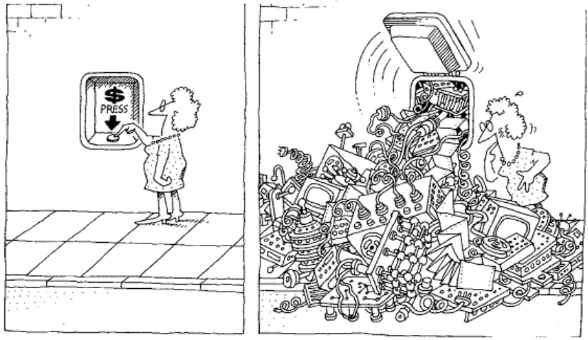
\includegraphics[width=0.5\textwidth]{complexityHiding.png}
        \end{center}
        \attribution{G. Booch, ``Object-oriented analysis and design''}
    \end{frame}

    \begin{frame}
        \frametitle{Свойства сложных систем}
        \begin{itemize}
            \item Иерархичность --- свойство системы состоять из иерархии подсистем или компонентов
            \begin{itemize}
                \item Декомпозиция
            \end{itemize}
            \item Наличие относительно небольшого количества видов компонентов, экземпляры которых сложно связаны друг с другом
            \begin{itemize}
                \item Выделение общих свойств компонентов, абстрагирование
            \end{itemize}
            \item Сложная система, как правило, является результатом эволюции простой системы
            \item Сложность вполне может превосходить человеческие интеллектуальные возможности
        \end{itemize}
    \end{frame}

    \begin{frame}
        \frametitle{Подходы к декомпозиции}
        \begin{itemize}
            \item Восходящее проектирование
            \begin{itemize}
                \item Сначала создаём ``кирпичики'', потом собираем из них всё более сложные системы
            \end{itemize}
            \item Нисходящее проектирование
            \begin{itemize}
                \item Постепенная реализация модулей
                \item Строгое задание интерфейсов
                \item Активное использование ``заглушек''
                \item Модули
                \begin{itemize}
                    \item Четкая декомпозиция
                    \item Минимизация
                    \item Один модуль --- одна функциональность
                    \item Отсутствие побочных эффектов
                    \item Независимость от других модулей
                    \item Принцип сокрытия данных
                \end{itemize}
            \end{itemize}
        \end{itemize}
    \end{frame}
    
    \begin{frame}
        \frametitle{Модульность}
        \begin{itemize}
            \item Разделение системы на компоненты
            \item Потенциально позволяет создавать сколь угодно сложные системы
            \item Строгое определение контрактов позволяет разрабатывать независимо
            \item Необходим баланс между количеством и размером модулей
        \end{itemize}
        \vskip 1cm
        \begin{center}
            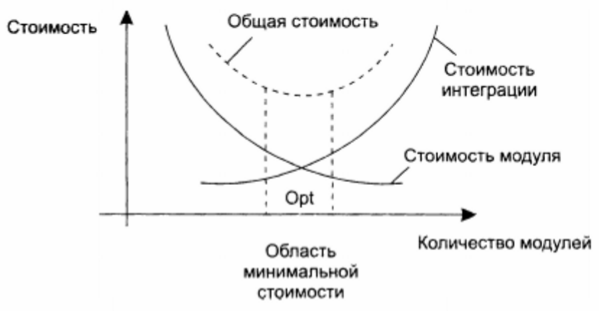
\includegraphics[width=0.5\textwidth]{modulesCost.png}
        \end{center}
    \end{frame}

    \begin{frame}
        \frametitle{Сопряжение и связность}
        \begin{itemize}
            \item \textbf{Сопряжение (Coupling)} --- мера того, насколько взаимозависимы разные модули в программе
            \item \textbf{Связность (Cohesion)} --- степень, в которой задачи, выполняемые одним модулем, связаны друг с другом
            \item Цель: слабое сопряжение и сильная связность
        \end{itemize}
    \end{frame}

    \section{Некоторые принципы ОО-проектирования}

    \begin{frame}
        \frametitle{Объекты}
        \begin{itemize}
            \item Objects may contain data, in the form of fields, often known as attributes; and code, in the form of procedures, often known as methods --- \textbf{\href{https://en.wikipedia.org/wiki/Object-oriented\_programming}{Wikipedia}}
            \item An object stores its state in fields and exposes its behavior through methods --- \textbf{\href{https://docs.oracle.com/javase/tutorial/java/concepts/object.html}{Oracle}}
            \item Each object looks quite a bit like a little computer --- it has a state, and it has operations that you can ask it to perform --- \textbf{\href{http://amzn.to/1PBmQpm}{Thinking in Java}}
            \item An object is some memory that holds a value of some type --- \textbf{\href{http://amzn.to/1XyGCtk}{The C++ Programming Language}}
            \item An object is the equivalent of the quanta from which the universe is constructed --- \textbf{\href{http://amzn.to/266oJr4}{Object Thinking}}
        \end{itemize}
    \end{frame}

    \begin{frame}
        \frametitle{Объекты}
        \begin{itemize}
            \item Имеют
            \begin{itemize}
                \item Состояние
                \begin{itemize}
                    \item Инвариант
                \end{itemize}
                \item Поведение
                \item Идентичность
            \end{itemize}
            \item Взаимодействуют через посылку и приём сообщений
            \begin{itemize}
                \item Объект вправе сам решить, как обработать вызов метода (\textbf{полиморфизм})
                \item Могут существовать в разных потоках
            \end{itemize}
            \item Как правило, являются экземплярами \textbf{классов}
        \end{itemize}
    \end{frame}

    \begin{frame}
        \frametitle{Абстракция}
        \textbf{Абстракция} выделяет существенные характеристики объекта, отличающие его от остальных объектов, с точки зрения наблюдателя
        \vskip 1cm
        \begin{center}
            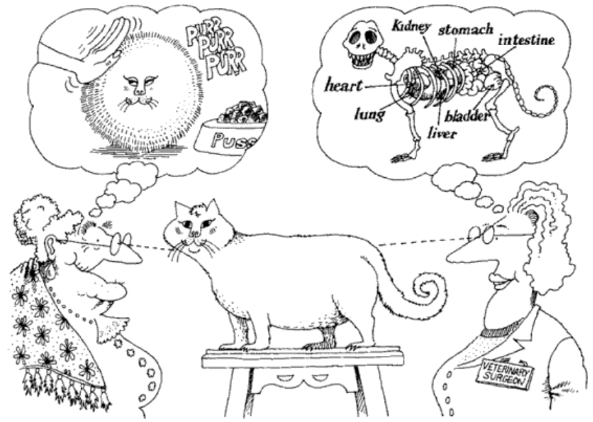
\includegraphics[width=0.45\textwidth]{abstraction.png}
        \end{center}
        \attribution{G. Booch, ``Object-oriented analysis and design''}
    \end{frame}

    \begin{frame}
        \frametitle{Инкапсуляция}
        \textbf{Инкапсуляция} разделяет интерфейс (\textbf{контракты}) абстракции и её реализацию

        Инкапсуляция защищает \textbf{инварианты} абстракции
        \vskip 1cm
        \begin{center}
            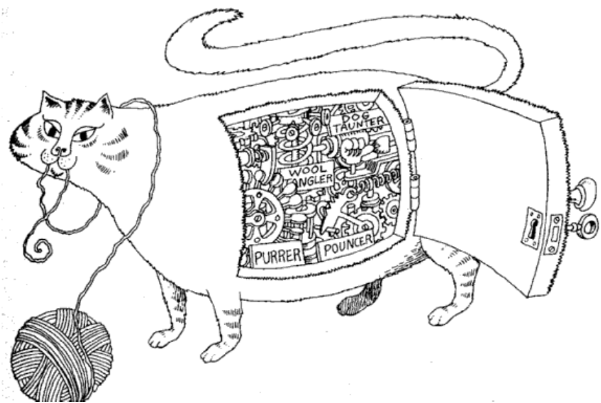
\includegraphics[width=0.45\textwidth]{incapsulation.png}
        \end{center}
        \attribution{G. Booch, ``Object-oriented analysis and design''}
    \end{frame}

    \begin{frame}
        \frametitle{Наследование и композиция}
        \begin{itemize}
            \item \textbf{Наследование}
            \begin{itemize}
                \item Отношение ``Является'' (is-a)
                \item Способ абстрагирования и классификации
                \item Средство обеспечения полиморфизма
            \end{itemize}
            \item \textbf{Композиция}
            \begin{itemize}
                \item Отношение ``Имеет'' (has-a)
                \item Способ создания динамических связей
                \item Средство обеспечения делегирования
            \end{itemize}
            \item Более-менее взаимозаменяемы
            \begin{itemize}
                \item Объект-потомок на самом деле включает в себя объект-предок
                \item Композиция обычно предпочтительнее
            \end{itemize}
        \end{itemize}
    \end{frame}

    \begin{frame}
        \frametitle{Определение объектов реального мира}
        \framesubtitle{Объектная модель предметной области}
        \begin{itemize}
            \item Определение объектов и их атрибутов
            \item Определение действий, которые могут быть выполнены над каждым объектом (назначение ответственности)
            \item Определение связей между объектами
            \item Определение интерфейса каждого объекта
        \end{itemize}
        \begin{center}
            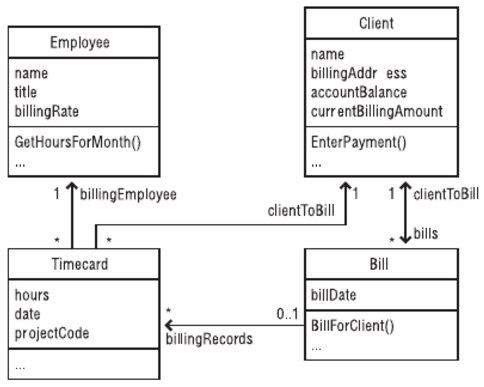
\includegraphics[width=0.35\textwidth]{billDomainModel.png}
        \end{center}
    \end{frame}

    \begin{frame}
        \frametitle{Изоляция сложности}
        \begin{columns}
            \begin{column}{0.6\textwidth}
                \begin{itemize}
                    \item Сложные алгоритмы могут быть инкапсулированы
                    \item Сложные структуры данных --- тоже
                    \item И даже сложные подсистемы
                    \item Надо внимательно следить за интерфейсами
                \end{itemize}
            \end{column}
            \begin{column}{0.4\textwidth}
                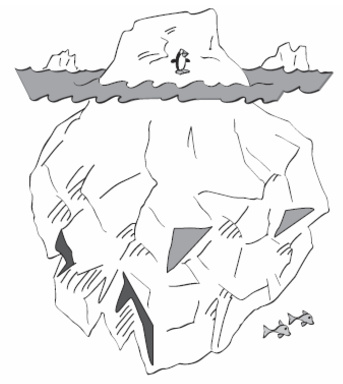
\includegraphics[width=0.7\textwidth]{complexity.png}
            \end{column}
        \end{columns}
    \end{frame}

    \begin{frame}
        \frametitle{Изоляция возможных изменений}
        \begin{itemize}
            \item Потенциальные изменения могут быть инкапсулированы
            \item Источники изменений
            \begin{itemize}
                \item Бизнес-правила
                \item Зависимости от оборудования и операционной системы
                \item Ввод-вывод
                \item Нестандартные возможности языка
                \item Сложные аспекты проектирования и конструирования
                \item Третьесторонние компоненты
                \item ...
            \end{itemize}
        \end{itemize}
    \end{frame}

    \begin{frame}
        \frametitle{Изоляция служебной функциональности}
        \begin{itemize}
            \item Служебная функциональность может быть инкапсулирована
            \begin{itemize}
                \item Репозитории
                \item Фабрики
                \item Диспетчеры, медиаторы
                \item Статические классы (\textit{Сервисы})
                \item ...
            \end{itemize}
        \end{itemize}
    \end{frame}

    \section{Принципы SOLID}
    
    \begin{frame}
        \frametitle{Принципы SOLID}
        \begin{itemize}
            \item Single responsibility principle
            \item Open/closed principle
            \item Liskov substitution principle
            \item Interface segregation principle
            \item Dependency inversion principle
        \end{itemize}
    \end{frame}

    \begin{frame}
        \frametitle{Single responsibility principle}
        \begin{itemize}
            \item Каждый объект должен иметь одну обязанность
            \item Эта обязанность должна быть полностью инкапсулирована в объект
        \end{itemize}
        \begin{flushright}
            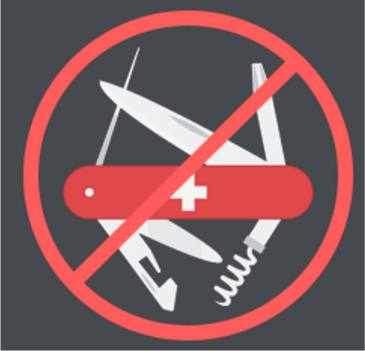
\includegraphics[width=0.25\textwidth]{singleResponsibility.png}
        \end{flushright}
    \end{frame}

    \begin{frame}
        \frametitle{Open/closed principle}
        \begin{itemize}
            \item Программные сущности (классы, модули, функции и т. п.) должны быть открыты для расширения, но закрыты для изменения
            \begin{itemize}
                \item Переиспользование через наследование
                \item Неизменные интерфейсы
            \end{itemize}
        \end{itemize}
        \begin{flushright}
            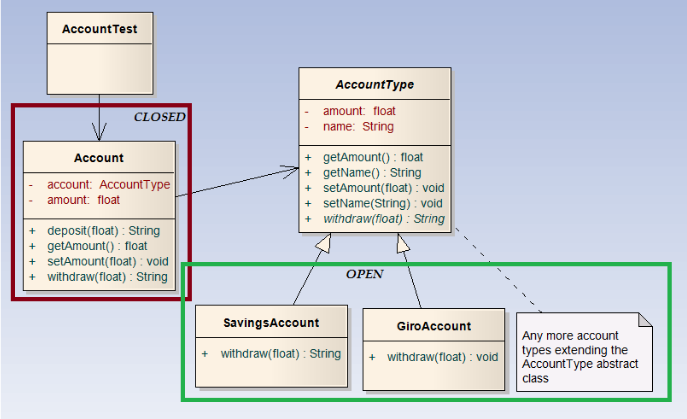
\includegraphics[width=0.5\textwidth]{openClosedPrinciple.png}
        \end{flushright}
    \end{frame}

    \begin{frame}
        \frametitle{Liskov substitution principle}
        \begin{itemize}
            \item Функции, которые используют базовый тип, должны иметь возможность использовать подтипы базового типа, не зная об этом
        \end{itemize}
        \begin{flushright}
            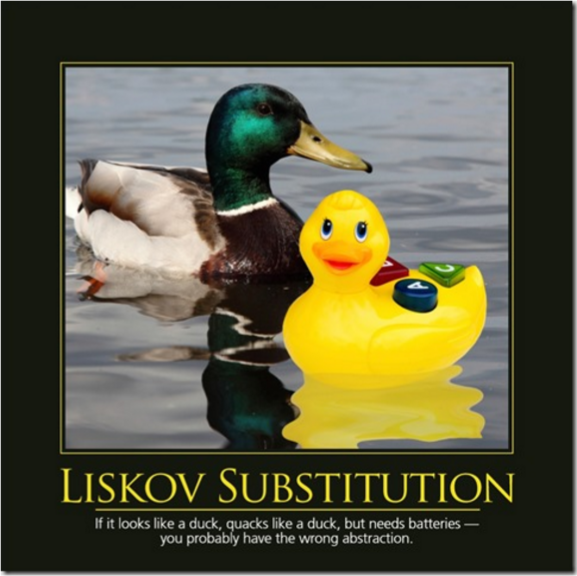
\includegraphics[width=0.4\textwidth]{liskovSubstitutionPrinciple.png}
        \end{flushright}
    \end{frame}

    \begin{frame}
        \frametitle{Interface segregation principle}
        \begin{itemize}
            \item Клиенты не должны зависеть от методов, которые они не используют
            \begin{itemize}
                \item Слишком ``толстые'' интерфейсы необходимо разделять на более мелкие и специфические
            \end{itemize}
        \end{itemize}
        \begin{flushright}
            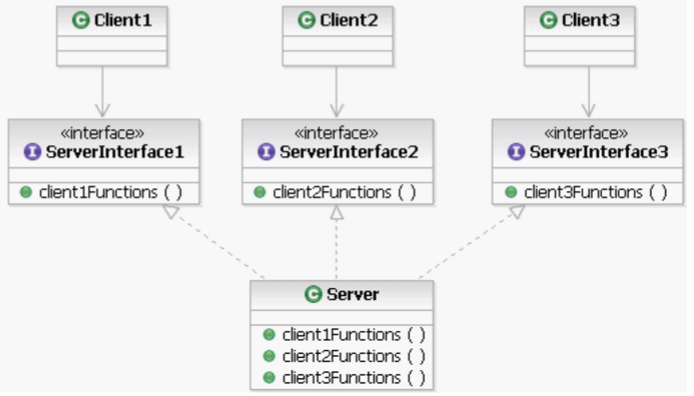
\includegraphics[width=0.5\textwidth]{interfaceSegregationPrinciple.png}
        \end{flushright}
    \end{frame}

    \begin{frame}
        \frametitle{Dependency inversion principle}
        \begin{itemize}
            \item Модули верхних уровней не должны зависеть от модулей нижних уровней. Оба типа модулей должны зависеть от абстракций
            \item Абстракции не должны зависеть от деталей. Детали должны зависеть от абстракций
        \end{itemize}
        \begin{flushright}
            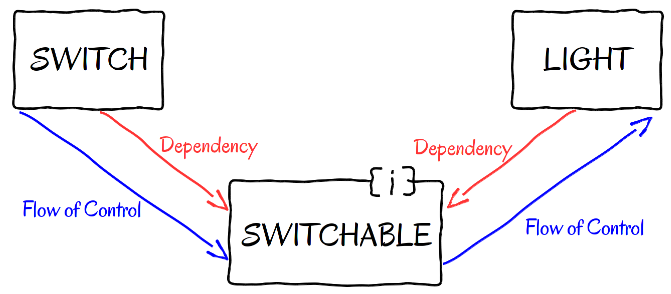
\includegraphics[width=0.5\textwidth]{dependencyInversionPrinciple.png}
        \end{flushright}
    \end{frame}

    \section{Закон Деметры}

    \begin{frame}
        \frametitle{Закон Деметры}
        \begin{itemize}
            \item ``Не разговаривай с незнакомцами!''
            \item Объект A не должен иметь возможность получить непосредственный доступ к объекту C, если у объекта A есть доступ к объекту B, и у объекта B есть доступ к объекту C
            \begin{itemize}
                \item \mintinline{java}|book.pages.last.text|
                \item \mintinline{java}|book.pages().last().text()|
                \item \mintinline{java}|book.lastPageText()|
            \end{itemize}
            \item Иногда называют ``Крушение поезда''
        \end{itemize}
        \begin{flushright}
            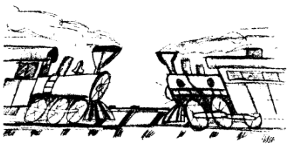
\includegraphics[width=0.35\textwidth]{trains.png}
        \end{flushright}
        \vspace{-0.8cm}
        \attribution{Р. Мартин, ``Чистый код''}
    \end{frame}

\end{document}
